\section{Introduction and Motivation}\label{sec:introduction}
In the era of Information Technology, the usage of software and its applications is continuously increasing and has become an important part of our lives. This makes the software industry one of the largest industries in the world and many companies are built around the development of software. With the growing usage of software, the software development process has changed drastically and has become more solution-oriented. Nowadays, the entire focus is on making the software development process fast, less complex, and more human-friendly. 
\newline\newline One of the approaches to reducing the complexity of software development is abstraction and separation of concerns \cite{modeltransform}. In recent times, (software) modeling has become an effective way of implementing this principle. In a traditional approach, developers manually write programs and check the specifications based on software models, which is often costly, incomplete, informal, and carries a major risk of failure. In contrast, model-driven software development (referred to as \textbf{MDSD} from now on) improves the way software is built by moving the focus from programming language code to representing the essential aspects of software in the form of software models. It reduces development costs and increases the reusability and maintainability of software. The objective of MDSD \cite{modeltransform} is to increase productivity and reduce time-to-market by enabling development at a higher level of abstraction and by using concepts closer to the problem domain at hand, rather than what is directly offered by programming languages. 
\newline\newline The core idea of the MDSD approach is based on models, modeling and model transformations. In this approach, developers represent real world systems as models at a suitable level of abstraction. Different models can be used to represent different views of a system.  Although these views are separate and result in models that can be independently manipulated by different developers, there are still numerous relations between models that must be taken into account to ensure that the entire system, described by the state of all models, is consistent. This phenomenon is handled by model transformation and certainly increases the developers productivity and quality of the models.

\textit{Bidirectional transformation} (referred to as \textbf{bx} from now on) is a technique used to synchronize two (or more) models. Such models are related, but don't necessarily contain the same information. Changes in one model can thus lead to changes in other models \cite{bx-grace}.
\newline\newline\textit{Bidirectional transformation} is used to deal with scenarios like\cite{bx-theoryandappl}:
\begin{itemize}
	\item {change propagation to the user interface as a result of underlying data changes}	
	\item {synchronization of business/software models}
	\item {refreshable data-cache incase of database changes}
	\item {consistency management between two artifacts by avoiding data loss}
\end{itemize}
The bx community (\url{http://bx-community.wikidot.com/}) has been doing research in many fields including software development, databases, mathematics and much more, to increase awareness for bx \cite{bx-grace}\cite{bx-dagstuhl}. As a result, many kinds of bx tools are being developed. These bx tools are based on various approaches, such as graph transformations e.g., eMoflon \cite{emoflon-part4}, bidirectionalization e.g., BIGUL \cite{bigul}, constraint solving e.g., Echo \cite{echo} and can be used in different areas of application \cite{bx-community}.

\subsection{Problem Statement}\label{subsec:probstmt}
\textit{Bidirectional transformation} is an emerging concept. In the past, many efforts have been made by conducting international workshops, seminars and through experiments conducted by developers / bx community to identify its potential. Also, in addition to the development of bx tools and bx language, benchmarks are being created for bx tools for systematic comparison \cite{benchmark-BX}.
\newline\newline  Although a significant amount of work has been done on bx but a general awareness and understanding for basic concepts, the involved challenges, and reasonable expectations is not really given. Hence, there exist conceptual and practical challenges with building software systems using bx-tools and as a result bx tools and their applicability is still not widely known and used \cite{bx-theoryandappl}.
\newline\newline From experience with working with master students (future software developers in industry), we have identified a set of bx learning goals that can be targeted to improve the situation.
Achieving these learning goals is, however, challenging as current possibilities (virtual machines, handbooks, etc) are either tool specific or ineffective because installation process to get the tool running is a time consuming process and sometimes requires technical expertise in a specific area/tool/programming language. In this fast paced world, people don't really want to spend much time in a process if it involves complexity and time consuming. Even after you get the tool running, it doesn't help in understanding the bx concepts and its corresponding technological space in use because of lack of proper explanations.

\subsection{Contribution}\label{subsec:contribution}
To solve the problems as described in Section \ref{subsec:probstmt}, in this thesis, my goals are as follows:
\begin{itemize} 
\item {Design and implement an interactive demonstrator.} 
\item {Spreading the basic concepts of bx to a wide audience and making them accessible and understandable.}
\end{itemize}
An existing bx tool will be used as a part of the demonstrator to realize \textit{bidirectional transformation}. The final prototype will be interactive and easily accessible to users to help them understand the potential, power and limitations of bx.
\newline\newline My approach for providing a solution to the problems described in Section \ref{subsec:probstmt}  consists of various stages which focuses on designing and implementing a successful bx tool demonstrator as shown in figure~\ref{fig:Approach_Overview}. 

\begin{figure}
	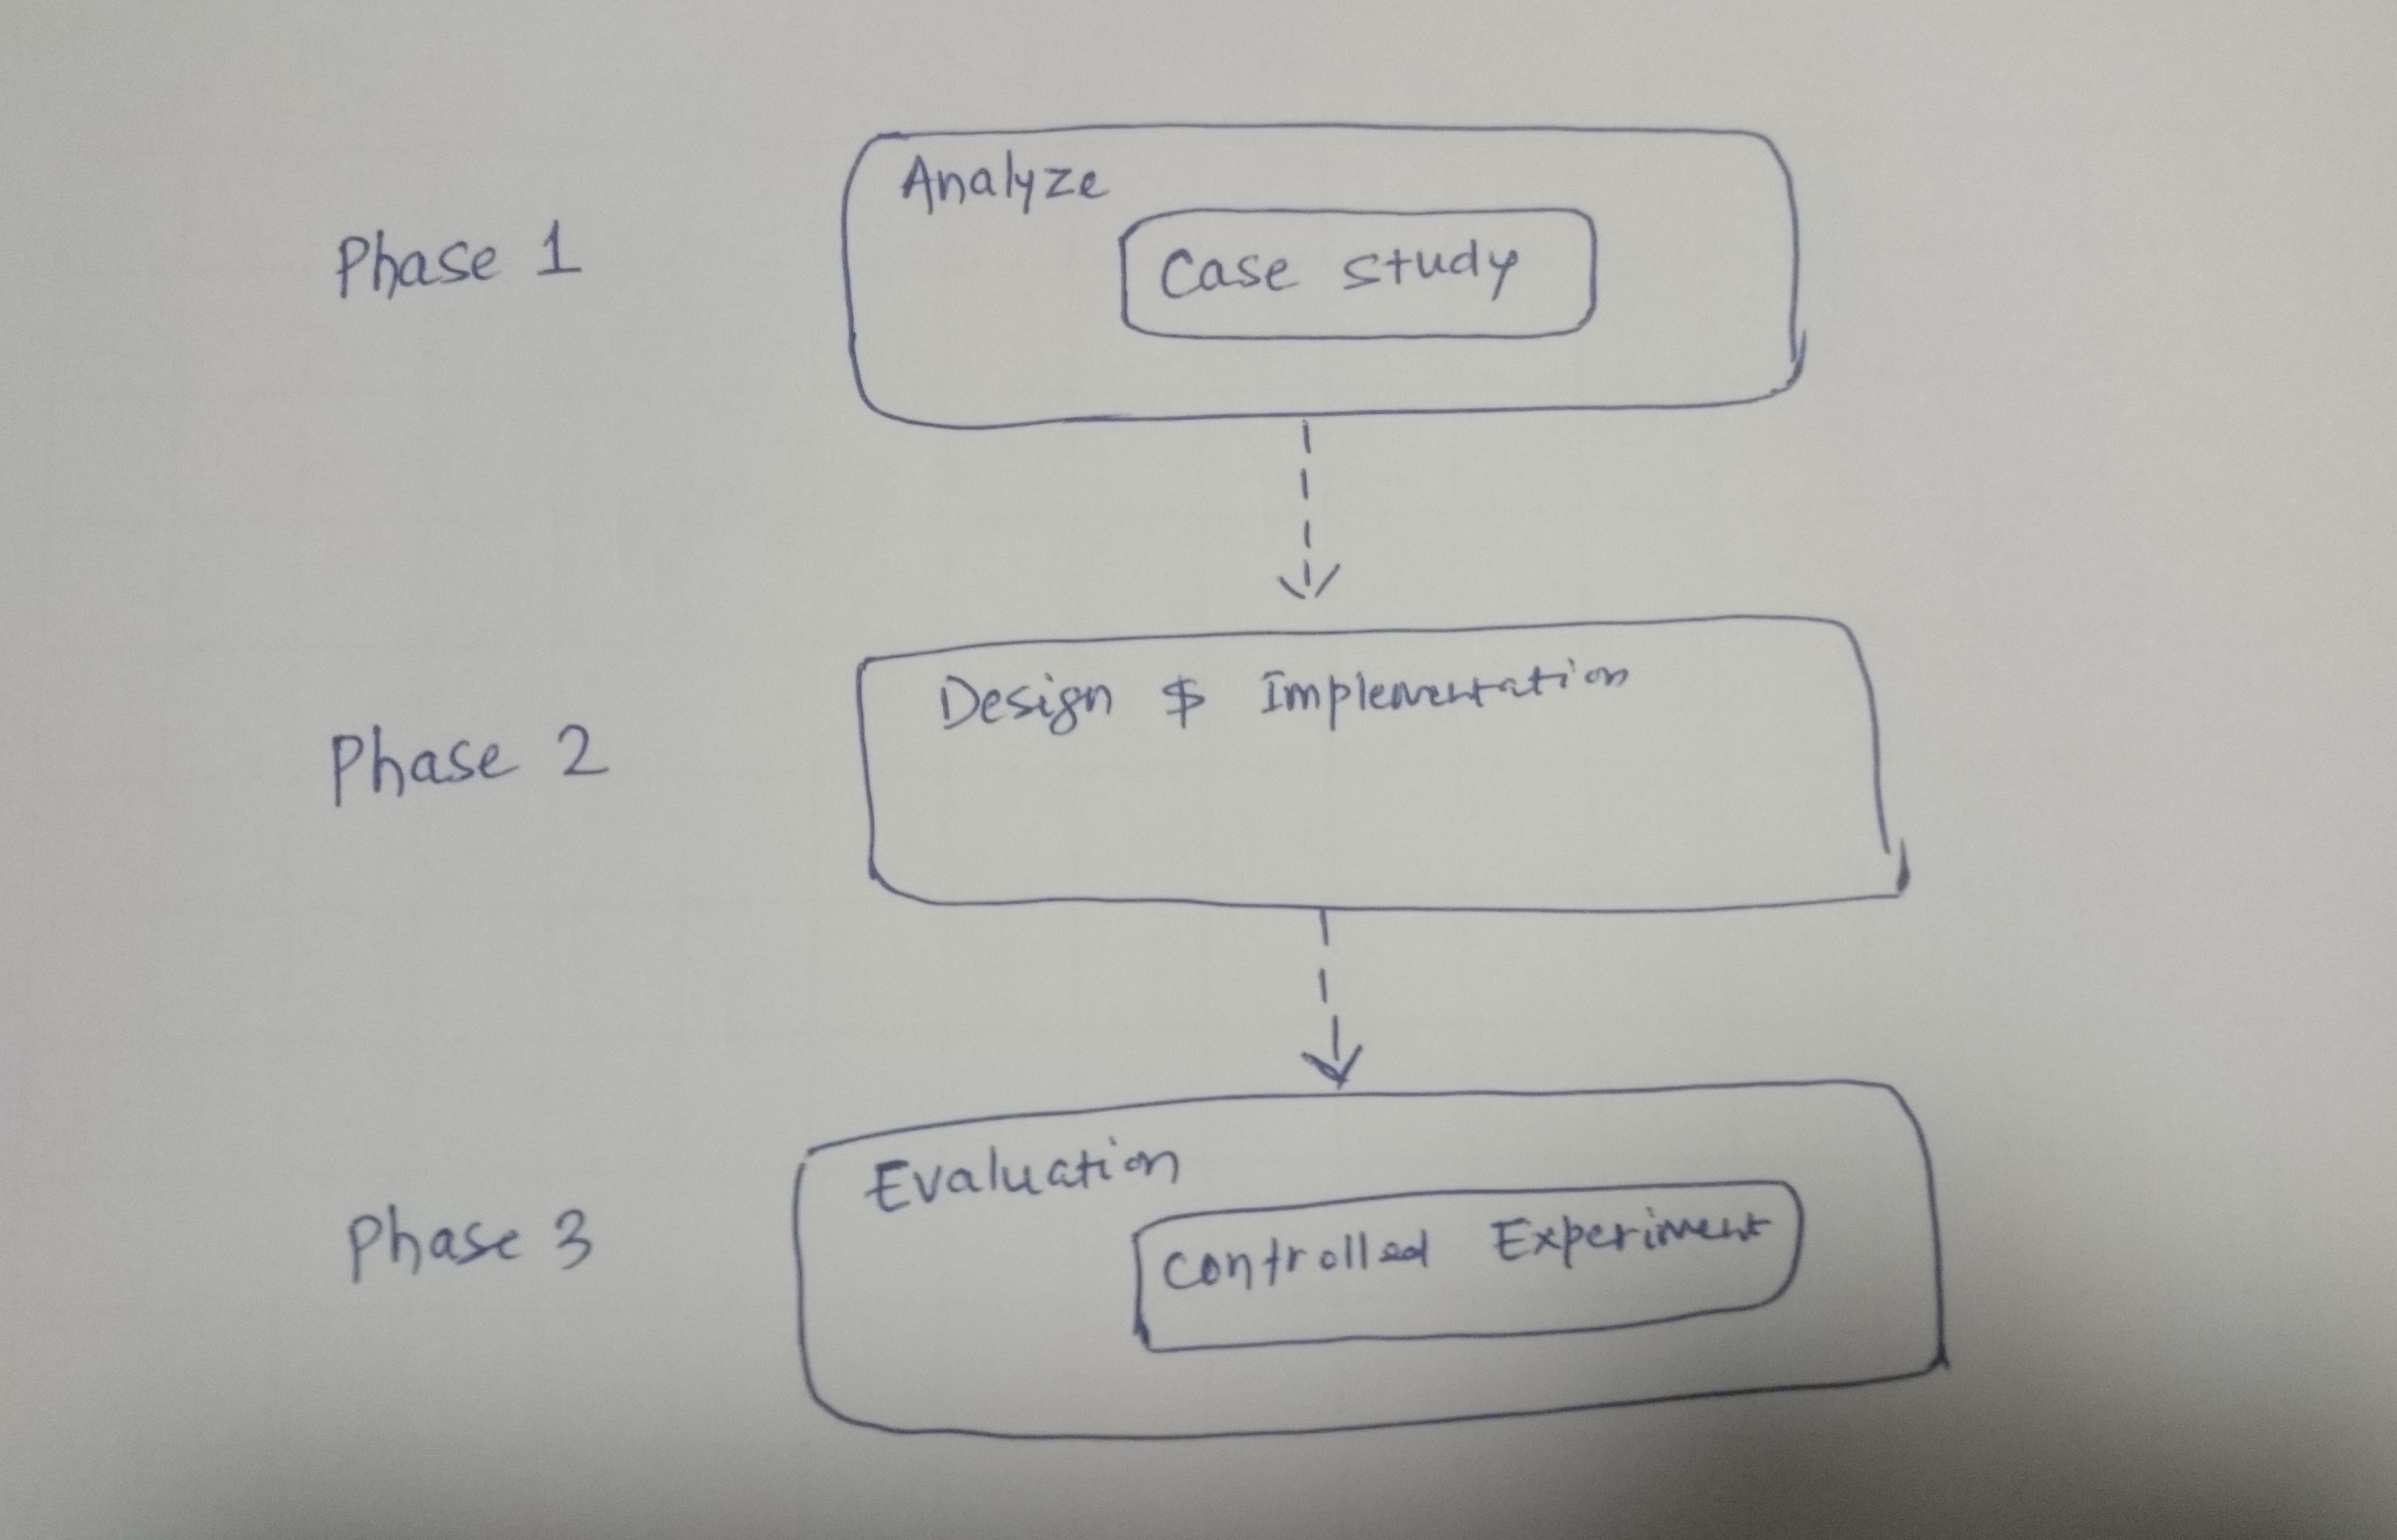
\includegraphics[width=1\textwidth]{figures/Approach_Overview}
	\caption{Approach Overview}
	\label{fig:Approach_Overview}
\end{figure}

\paragraph{Analysis}
This stage is based on the research method called Case Study \cite{semethods}. In any research, there could be many cases and each case could focus on a number of different research questions, each of which leads to a different direction in developing solution strategies \cite{semethods}. Hence, this method aims at selecting cases that are most relevant to the research and research questions are pinned down to the exact problems in hand. 
\newline\newline Initially, the case study was based on the existing work/research done on bx, existing tools available in the market, flexibility in usage, time and technical expertise required to use these bx tools, and the implementation of these tools in different areas. With the initial study and knowledge gathered, I had formulated the following associated research questions (referred to as \textbf{RQ} from now on):
\begin{itemize}
\item {\textbf{\textit{RQ1}} -- What are the core requirements for implementing a successful bx demonstrator ?}
\item {\textbf{\textit{RQ2}} -- What kind of interactivity and to what extent is it required in the bx demonstrator ?}
\item {\textbf{\textit{RQ3}} -- Which goals can be particularly well addressed in a bx demonstrator and why ?}
\item {\textbf{\textit{RQ4}} -- To what extent is such a bx demonstrator reusable?}
\\RQ4 can be split into the following sub-questions:
\\\textbf{\textit{RQ4.1}} -- Is the implementation of the demonstrator bx tool-specific ?
\\\textbf{\textit{RQ4.2}} -- Is the implementation of the demonstrator example-specific?
\item {\textbf{\textit{RQ5}} -- Is it possible to teach the concepts of bx through a demonstrator ?}
\item {\textbf{\textit{RQ6}} -- Does an interactive GUI helps an user to increase his/her understanding of bx concepts ?}
\end{itemize}
All of my work is directly or indirectly related to the above research questions.

\paragraph{Design and Implementation}
This stage is consist of all the steps related to designing and implementing the demonstrator by keeping a focus on the research questions.
\newline\newline First, I have constructed a few examples which can be implemented covering the requirements and showing the usability of bx tools through demonstrator. Then, taking account the availabilities of resources and usability factor, I finally chose the best suitable example to implement and build the final prototype. Section \ref{subsec:exampleforimplementation} describes list of all the examples.
\newline\newline Second step was to choose a bx-tool for my demonstrator. Based on the gathered information and taking account implementation related issues, I have chosen a bx-tool to be used as a part of the demonstrator to realize bx. Section \ref{subsec:bxtoolselection} explains the process in detail.
\newline\newline Next step was to set up the entire application framework for implementing the demonstrator. First, I did some research by going through materials on software design patterns and web application architecture. Then, I prepared a few proof of concepts(POC) for checking the feasibilty of the architecture designs before finalising my application framework. Section \ref{subsec:architecturedesign} explains the process in detail.

\paragraph{Evaluation} 
This stage is based on the research method called Controlled Experiments \cite{semethods}. This experiment is based on one or more hypothesis, which guide all steps of the experimental design, deciding which variables to include and how to measure them. So, it is an investigation of one or more hypothesis where one or more independent variables are manipulated to measure their effect on one or more
dependent variables. Learning goals were prepared along with the scenarios to explain them and questions were asked on these concepts to different groups of participants. Finally, data is collected and analyzed to measure the outcome. Section \ref{sec:evaluation} explains the process in detail.

\subsection{Structure of Thesis}\label{subsec:structure}
This document is structured as follows: 

Chapter 1 (introduction) contains the introduction and motivation about the thesis with a solution strategy. Chapter 2 discusses the related terminologies with respect to bidirectional transformation. Chapter 3 describes the requirements for implementing a successful bx demonstrator. Chapter 4 explains the related work that has been done on bx in last few years and the related problems. Chapter 5 describes all the high-level concepts of my implementation work in brief with related diagrams. Chapter 6 provides the in-depth details of each implementation layer along with UML diagrams. Chapter 7 presents a walkthrough of the application from UI perspective. Chapter 8 contains the feedback from user groups, evaluation results and learning goals(based on research questions). Last chapter summarizes all the work which was done as part of this thesis and draws useful conclusions followed by future work.

\section{Foundation}\label{sec:foundation}
This chapter provides an overview of my running example in Section \ref{subsec:runningexample} followed by definitions of some commonly used terminologies with respect to bx in Section \ref{subsec:definitions}. This chapter will lay the foundation for understanding the basics for the reader and will help him/her in apprehending the concepts explained in further chapters.

In this thesis, bidirectional transformation will be discussed by referring to a \textit{Kitchen Model} and a \textit{Grid Model} of a software system. Both the models describes the structure and behaviour of the real system "kitchen" but from different perspectives.

\subsection{Running Example}\label{subsec:runningexample}
This example is a simplified kitchen planner. Figure~\ref{fig:Running_Example_GUI} describes the relation between the \textit{Kitchen Model} denoted by \textit{Kitchen} (right-hand side canvas) and the \textit{Grid Model} denoted by \textit{Layout} (left-hand side canvas) from GUI point of view. 

\begin{figure}
	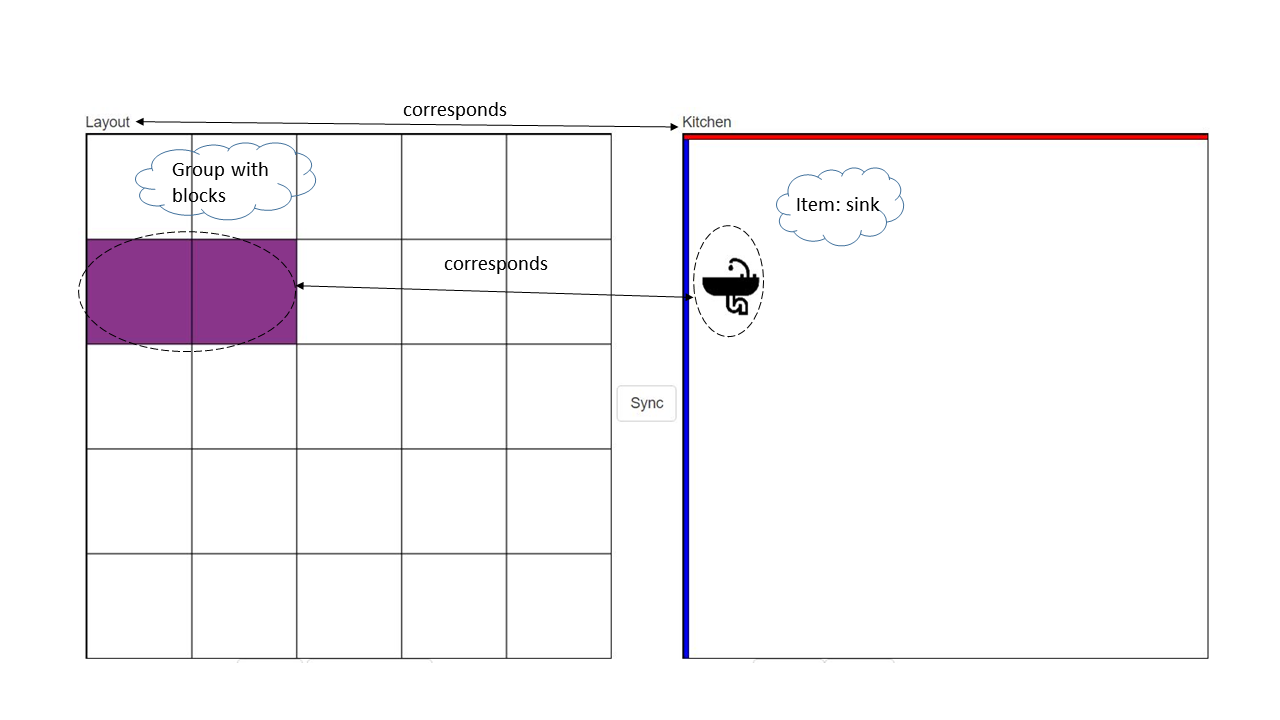
\includegraphics[width=1\textwidth]{figures/KitchenToGrid}
	\caption{Running Example: GUI}
	\label{fig:Running_Example_GUI}
\end{figure}

\begin{figure}
	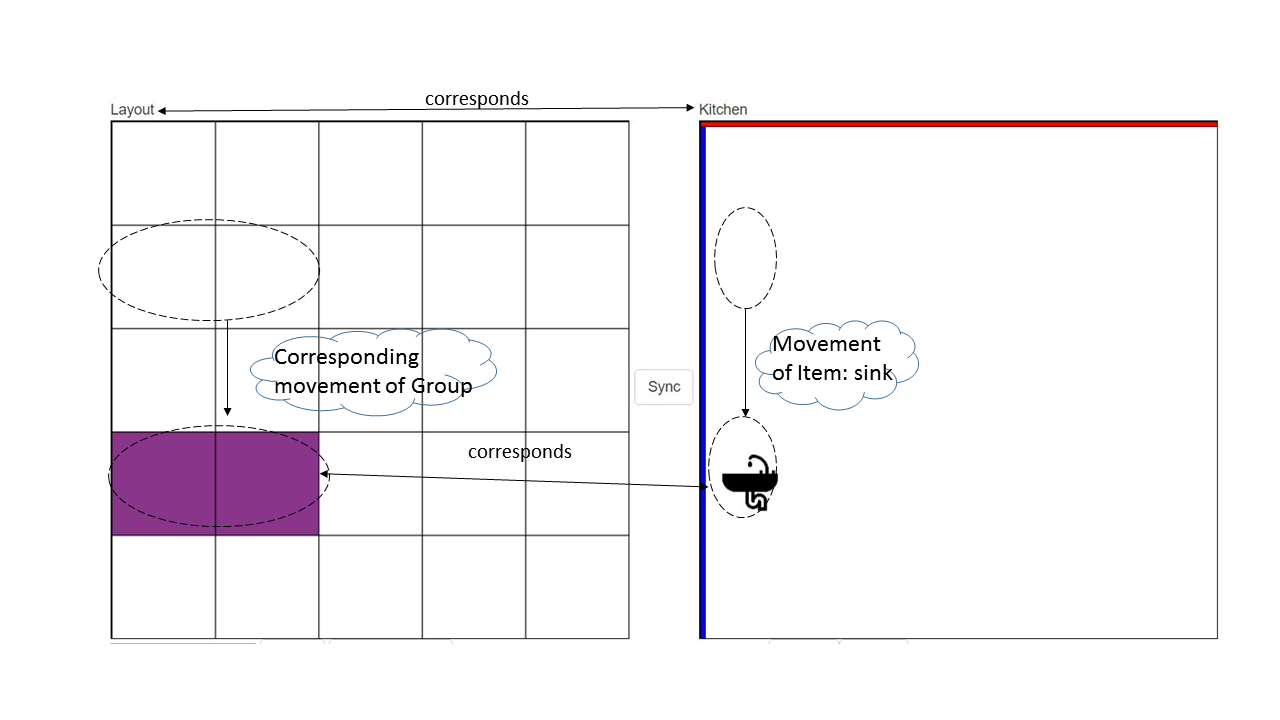
\includegraphics[width=1\textwidth]{figures/KitchenToGrid_consistency}
	\caption{Running Example: GUI (consistency preservation)}
	\label{fig:Running_Example_GUI_consistency}
\end{figure}

\textit{Kitchen} contains items e.g., sink, fridge, table etc. You can create, delete or move these items in the kitchen space, and press "Sync" to propagate your changes to the layout. The \textit{Layout} consist of groups with certain number of blocks. This shows how much space the objects occupy as coloured groups of blocks organised in a grid. Here, the \textit{Kitchen} corresponds to the \textit{Layout} and a \textit{Item} corresponds to a \textit{Group}. This is described by Figure~\ref{fig:Running_Example_GUI} where an item e.g., \textit{sink} created in the \textit{Kitchen} corresponds to a group in the \textit{Layout}.
\newline\newline Both artifacts are created and evolved together during the lifecycle of the application representing a kitchen workspace throughout. Thus, changes in one domain should be propagated to the other domain in order to ensure consistency between these related artifacts. This phenomenon is showed by Figure~\ref{fig:Running_Example_GUI_consistency}.
\newline\newline Model transformation and synchronization is discussed with this scenario throughout this thesis. 

\subsection{BX Basics}\label{subsec:definitions}
\paragraph{Definition 1} (\textit{Model and Meta-Model})\\
A model depicts the structure and/or behavior of a real system under discussion from a certain point of view and at a certain level of abstraction which helps in managing and understanding the complexities of a system \cite{uml} \cite{mdsd}. It is denoted as "M". Model cretion helps in keeping a clear focus on selected concepts and rules relevant for a particular concern and omitting irrelevant details.
\newline\newline A meta-model 
\newline\newline \textit{Example:} In my demonstrator, the example that I have implemented has two models i.e., \textit{Kitchen} and \textit{Grid}. Both the models represent the reality "Kitchen". A relation between reality and models is shown in Table~\ref{tab:Model_Reality}. Whereas, figure~\ref{fig:Abstract_KitchenModel} shows an abstract view of the \textit{Kitchen} model and figure~\ref{fig:Concrete_KitchenModel} depicts a concrete example of \textit{Kitchen} model.

\begin{table}
	\centering	
	\begin{tabular}{|p{3cm}|p{3cm}|p{9cm}|}
		\hline
		\rowcolor[gray]{.8}	
		\textbf{Reality} & \textbf{Model} & \textbf{Aspects Covered} \\
		\hline
		Kitchen & Kitchen Model & 
		\begin{itemize}
			\item Area of a kitchen as a white space
			\item 4 Walls of a kitchen
			\item contains the objeccts of a kichen
			\item Creation, Movement, Deletion of kitchen objects
		\end{itemize}\\
		\hline
		Kitchen & Grid Model & 
		\begin{itemize}
			\item Area of a kitchen as a block structure
			\item 4 Walls of a kitchen
			\item contains the objeccts of a kichen
			\item Creation, Deletion of kitchen objects
		\end{itemize}\\
		\hline					
		
	\end{tabular}
	\label{tab:Model_Reality}
	\caption{Model and Reality}
\end{table}

\begin{figure}
	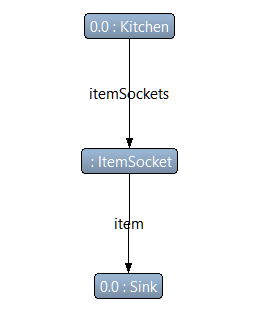
\includegraphics[width=0.5\textwidth]{figures/KitchenModel_Abstract}
	\caption{Abstract Kitchen Model}
	\label{fig:Abstract_KitchenModel}
\end{figure}

\begin{figure}
	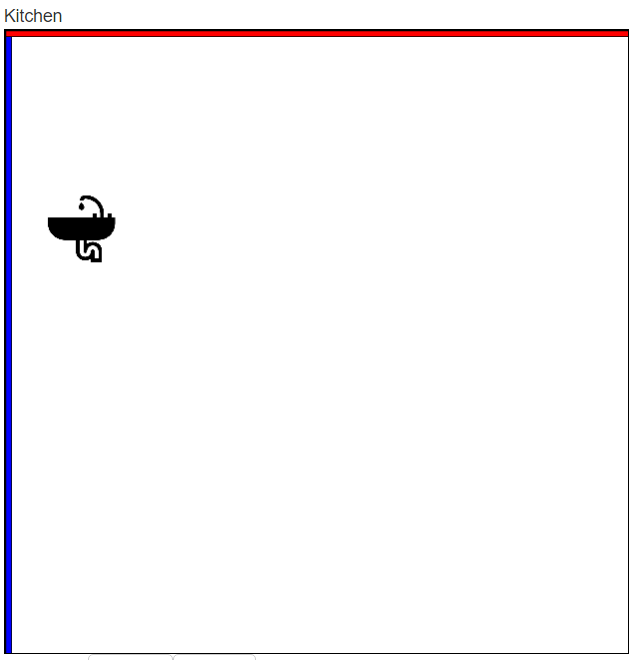
\includegraphics[width=0.5\textwidth]{figures/Kitchen_Concrete}
	\caption{Concrete Kitchen Model}
	\label{fig:Concrete_KitchenModel}
\end{figure}

\paragraph{Definition 2} (\textit{Modeling})\\
Modeling is the process which allows a developer to specify, visualize and capture a variety of important characteristics of a system in corresponding models which helps in decision making during development stages \cite{uml}. Nowadays, Unified Modeling Language (UML) \cite{uml} is used to visualize models in an object-oriented fashion.
\newline\newline\textit{Example:} In my demonstrator example, the process of identifying and constructing the "Kitchen Model" with the characteristics that is required for the task is an example of modeling. \textit{Kitchen} model contains three classes i.e., \textit{Kitchen}, \textit{Item Socket} and \textit{Item}. \textit{Kitchen} class contains \textit{itemSockets} and a \textit{Item Socket} class contains an \textit{item}. Figure~\ref{fig:Abstract_KitchenModel} shows an abstract view of the \textit{Kitchen} model 

\paragraph{Definition 3} (\textit{Delta})\\ 
Delta is the change done to one or more properties of an artefact. It denotes the relationships between models from the same model space \cite{benchmarx-reload}. It is denoted $\delta$: M $\longrightarrow$ M' where M' is an updated version of M.

\begin{table}
	\centering	
	\begin{tabular}{|p{5cm}|p{10cm}|}
		\hline
		\rowcolor[gray]{.8}	
		\textbf{Model} & \textbf{Delta ($\delta$)} \\
		\hline
		Kitchen Model & 
		\begin{itemize}
			\item Creating a new Item
			\item Deleting an existing Item
			\item Moving an Item
		\end{itemize}\\
		\hline				
		
	\end{tabular}
	\label{tab:Examples_of_Delta}
	\caption{Examples of Delta}
\end{table}

\begin{figure}
	
\includegraphics[width=1\textwidth]{figures/Delta_Abstract}
	\caption{Delta Propagation (Abstract Example)}
	\label{fig:DeltaPropagation_Abstract}
\end{figure}
\begin{figure}
	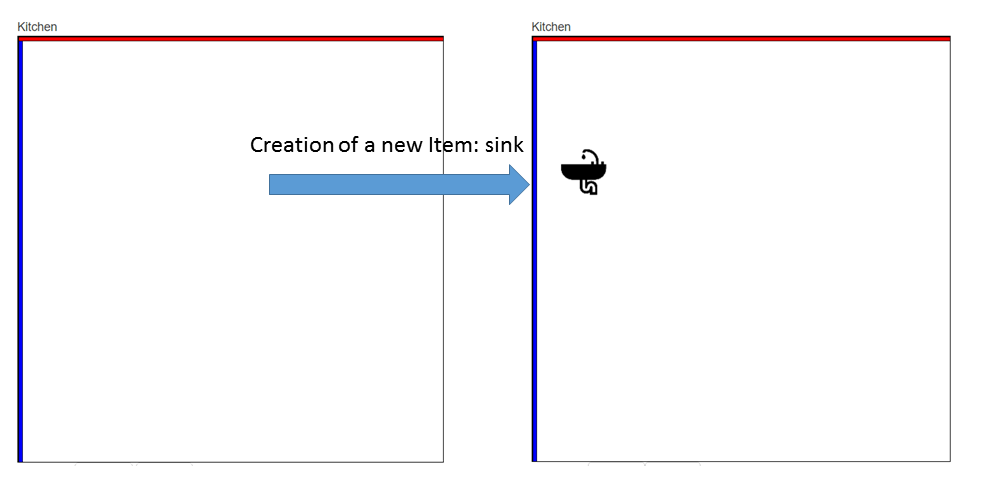
\includegraphics[width=1\textwidth]{figures/Delta_Concrete}
	\caption{Delta Propagation (Concrete Example)}
	\label{fig:DeltaPropagation_Concrete}
\end{figure}

\textit{Example:} In my demonstrator example, deltas related to the "Kitchen Model" are described in Table~\ref{tab:Examples_of_Delta}. Whereas, figure~\ref{fig:DeltaPropagation_Abstract} shows an abstract view of delta propagation and figure~\ref{fig:DeltaPropagation_Concrete} depicts a concrete example of delta propagation, where creation of a new item e.g., sink causes the updation from Kitchen to Kitchen'.

\paragraph{Definition 3.1} (\textit{Structural Delta})\\ 
Structural Delta denoted as "s-delta" is the collection of changes done to a model to update it, which is compatible with structure \cite{benchmarx-reload}. The way the changes are applied to the original model to result in a updated model (models of the same model space) don't necessarily have to be in the order in which they are performed. 

\paragraph{Definition 3.2} (\textit{Operational Delta})\\  
Operational Delta denoted as "o-delta" is the collection of operational specification changes done to a model to update it \cite{benchmarx-reload}. It is important that the changes are applied to the original model to result in a updated model (models of the same model space) have to be in the order in which they are performed. 

\paragraph{Definition 4} (\textit{Model Space})\\
Model Space describes all the states of an artefact and all the deltas which lead from one state to another.
\begin{figure}
	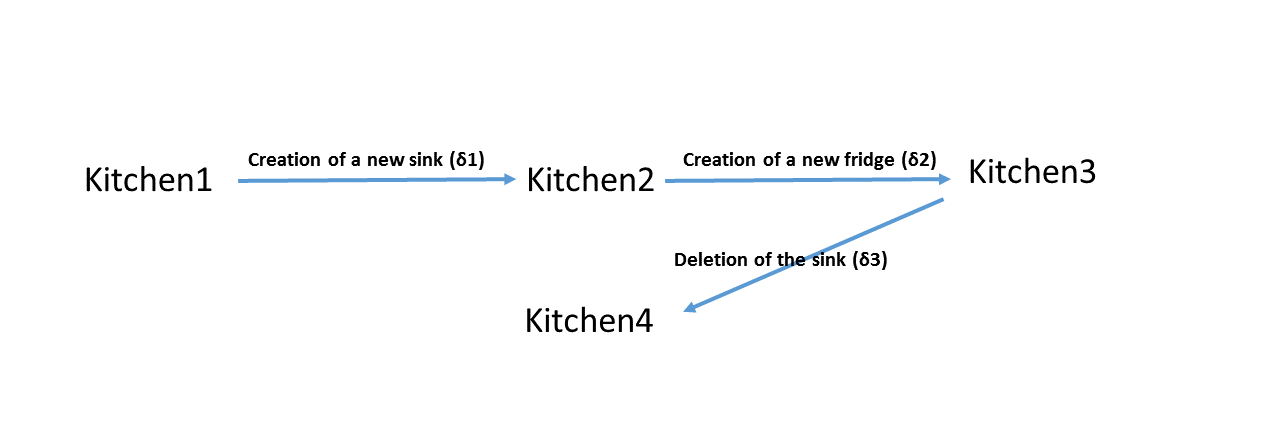
\includegraphics[width=1\textwidth]{figures/Model_Space}
	\caption{Model Space}
	\label{fig:Model_Space}
\end{figure}
\newline\newline\textit{Example:} In my demonstrator example, an concrete example of a model space is shown in figure~\ref{fig:Model_Space} with all the states i.e., Kitchen1, Kitchen2, Kitchen3, Kitchen4 along with its deltas i.e., $\delta$1, $\delta$2, $\delta$3 of the \textit{Kitchen} Model.

\paragraph{Definition 5} (\textit{Correspondence Links})\\
Relationships between models from different model spaces are called correspondence links, or just corrs \cite{benchmarx-reload}. A corr is a set of links  r(a; b) between elements (a in A, b in B), which are compatible with the models' structure and denoted by double bidirectional arrows, e.g., R: A $\Longleftrightarrow$ B. 
\newline\newline\textit{Example:} In my demonstrator example, an example of a corr is r(group; itemSocket) where \textit{group}, \textit{itemSocket} are the elements of \textit{Grid} and \textit{Kitchen} model respectively. Figure~\ref{fig:Correspondence_Links} shows a concrete example of the corr.
\begin{figure}
	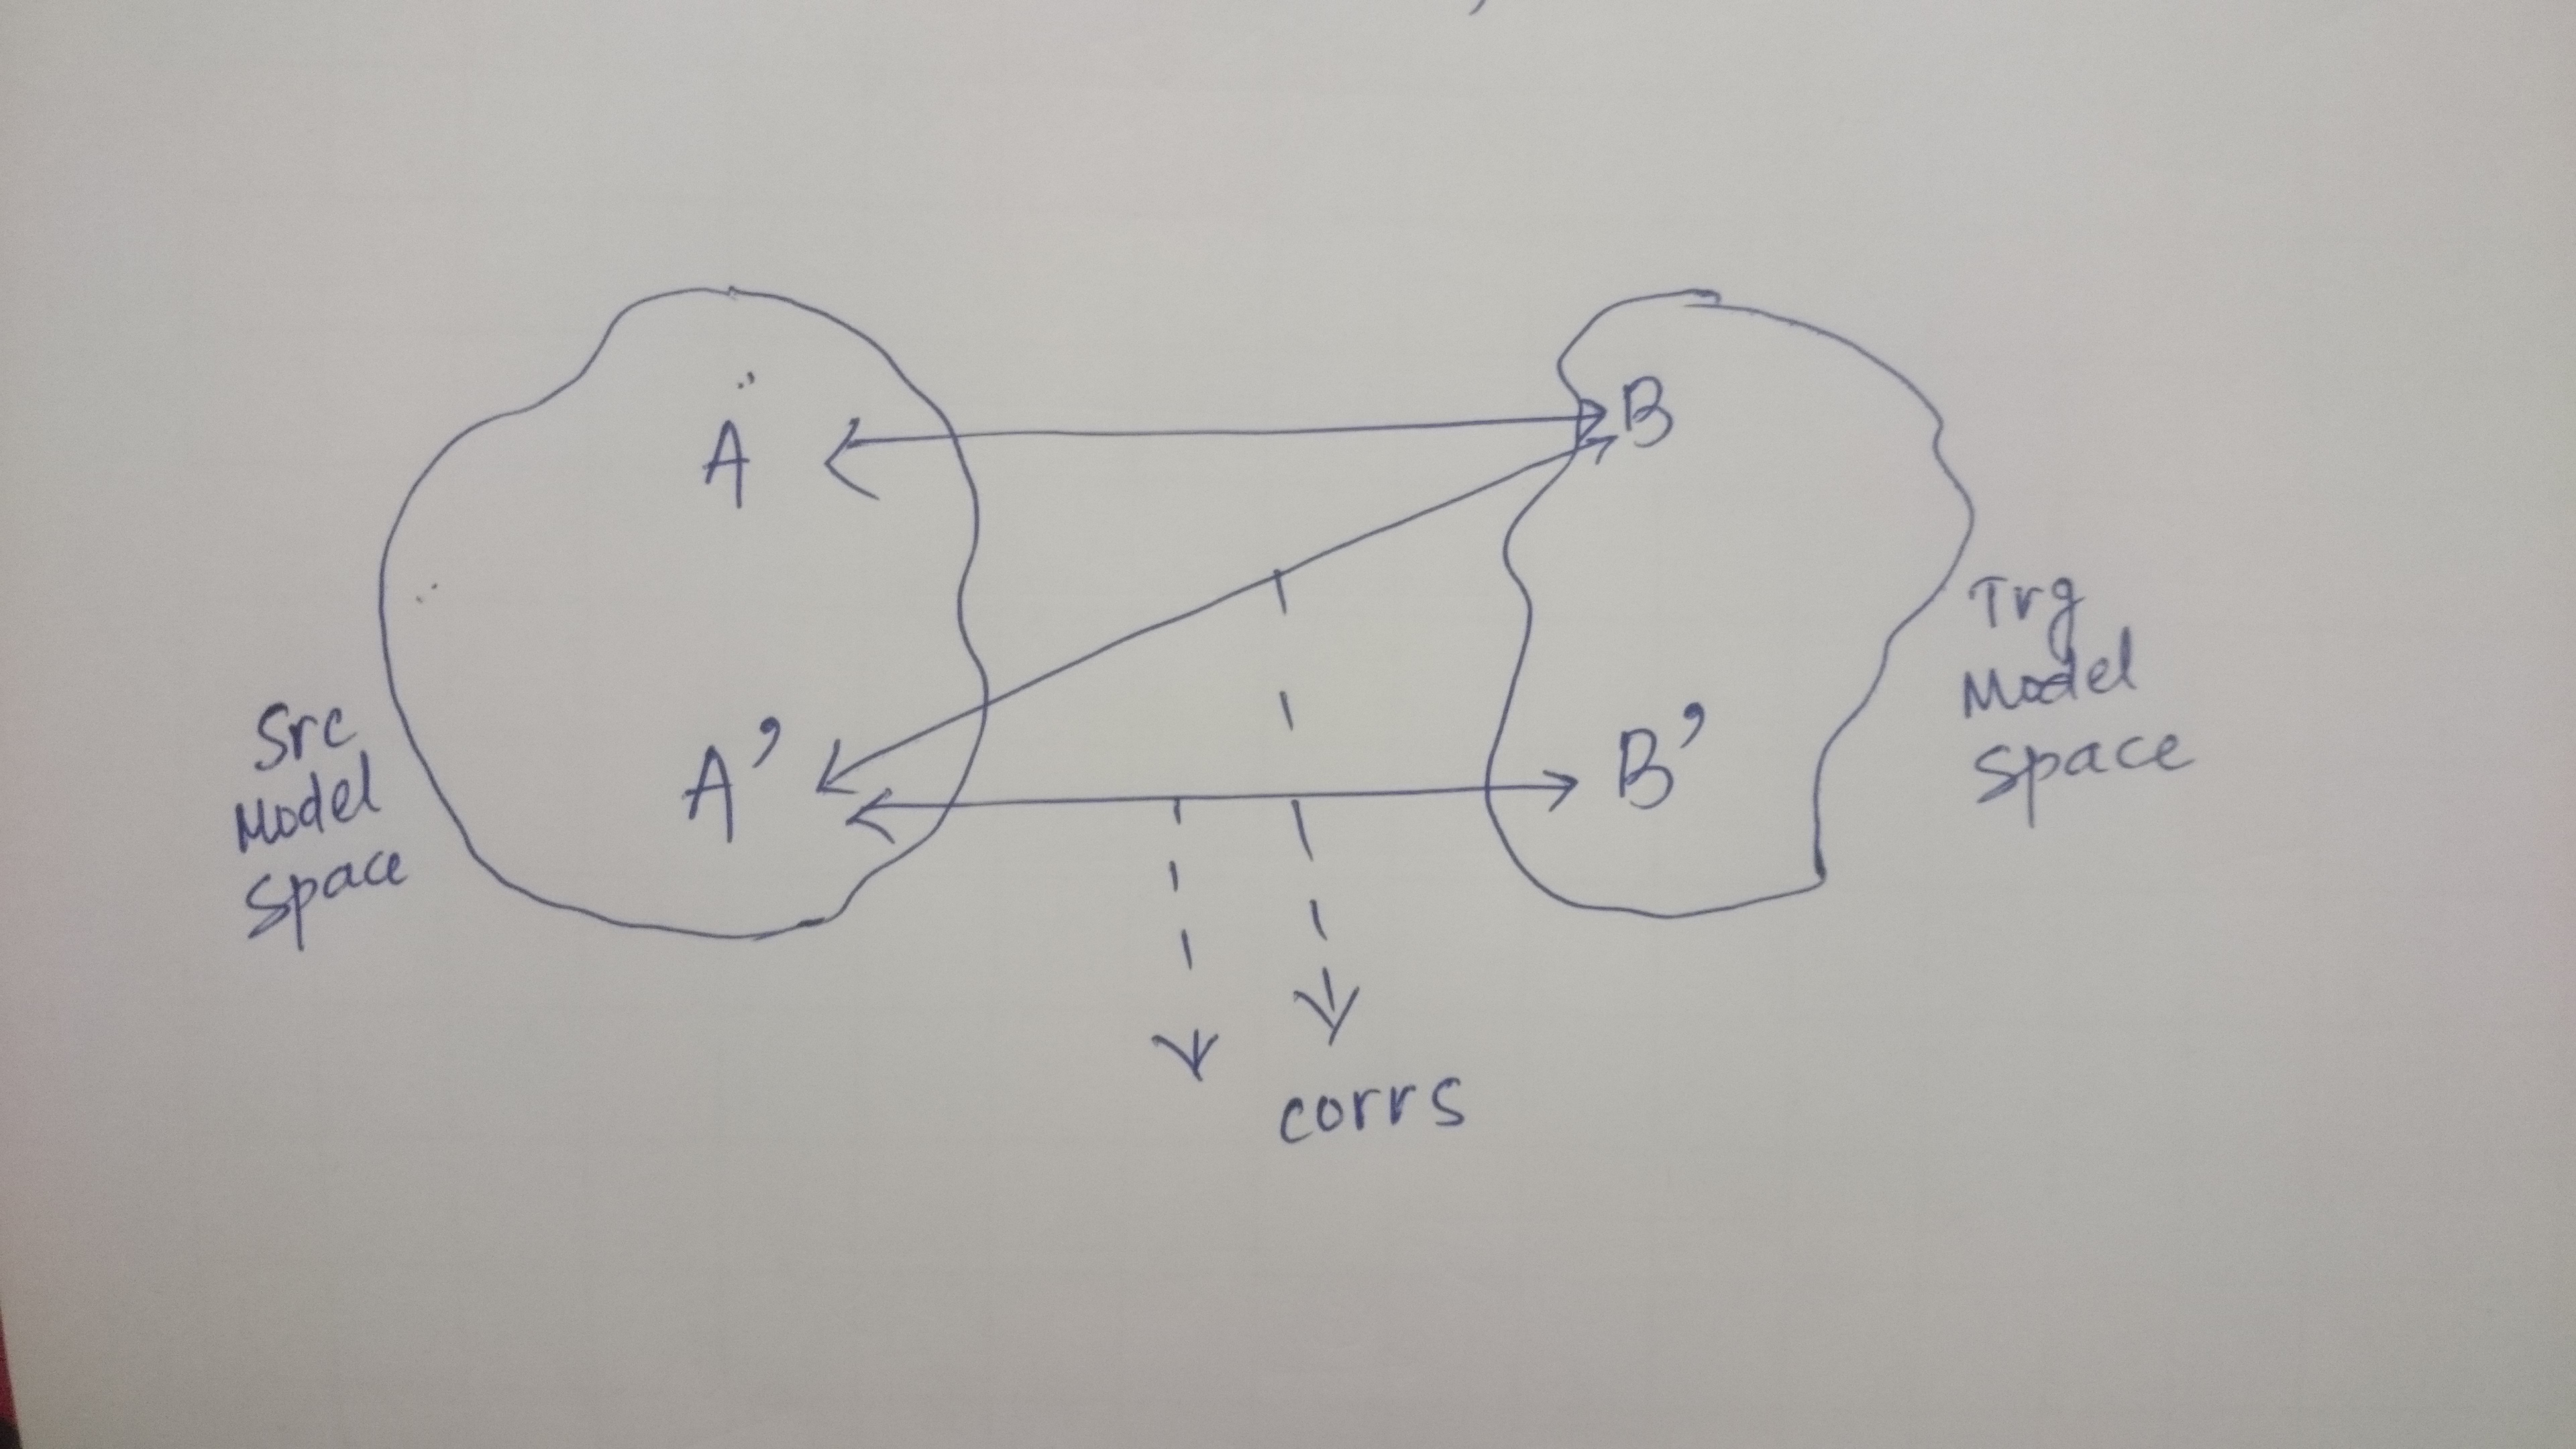
\includegraphics[width=1\textwidth]{figures/Corr}
	\caption{Correspondence Links}
	\label{fig:Correspondence_Links}
\end{figure}

\paragraph{Definition 6} (\textit{Transformation})\\
Transformation is the process in which takes one or more source models as input and produce one or more target models as output (models from different model spaces) expressed in either same abstraction level or in different abstraction level following a set of transformation rules \cite{modeltransform}. 

\begin{figure}
	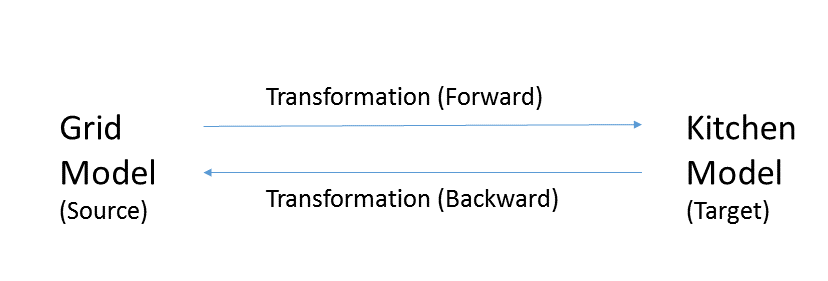
\includegraphics[width=1\textwidth]{figures/Transformation_Abstract}
	\caption{Transformation (Abstract Diagram)}
	\label{fig:Transformation_Abstract}
\end{figure}

\paragraph{Definition 6.1} (\textit{Forward Transformation})\\
Forward Transformation is the transformation from the \textit{Source} model to the \textit{Target} model.

\paragraph{Definition 6.2} (\textit{Backward Transformation})\\ 
Backward Transformation is the transformation from the \textit{Target} model to the \textit{Source} model.
\newline\newline\textit{Example:} In my demonstrator example, "Grid Model" is the \textit{Source} model and "Kitchen Model" is the \textit{Target} model. Forward transformation will cause "Grid Model" to transform into "Kitchen Model" and Backward transformation will cause "Kitchen Model" to transform into "Grid Model". Figure~\ref{fig:Transformation_Abstract} shows an abstract example of the transformation process and figure~\ref{fig:Transformation_Concrete} depicts a concrete example of the transformation process describing both forward and backward transformation.

\begin{figure}
	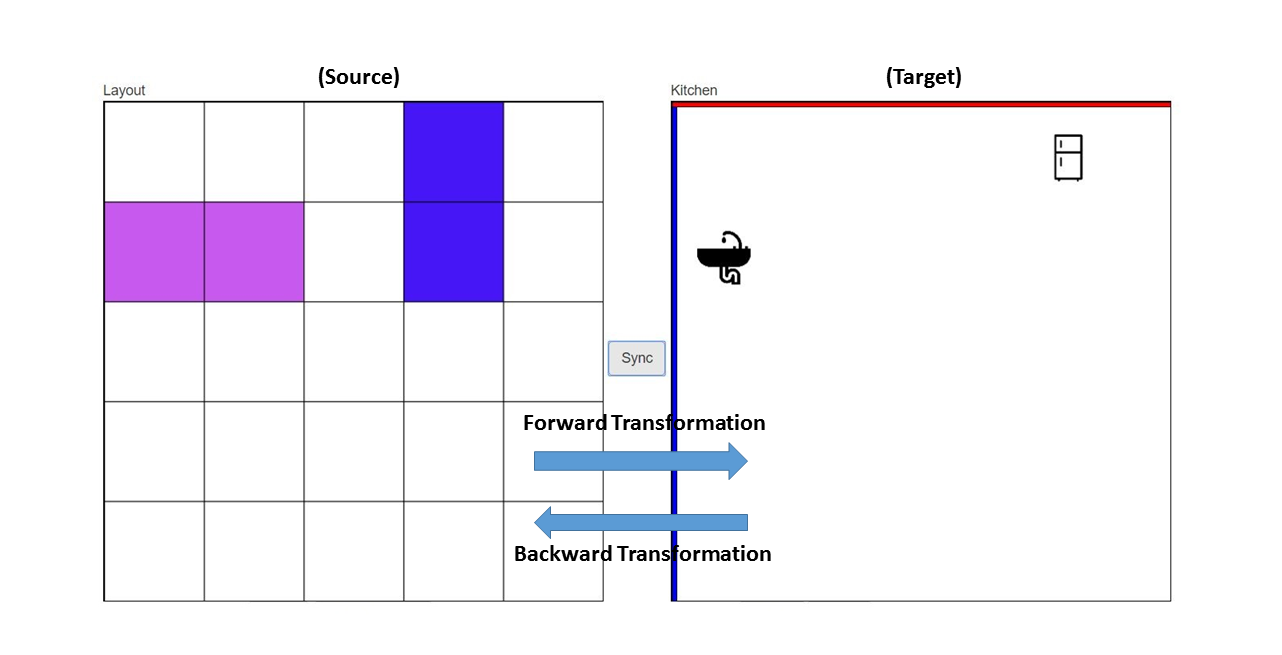
\includegraphics[width=1\textwidth]{figures/Transformation_Concrete}
	\caption{Transformation (Concrete Diagram)}
	\label{fig:Transformation_Concrete}
\end{figure}

\paragraph{Definition 7} (\textit{Consistency})\\ 
Changes in one model may or may not cause any change in other model (models from different model spaces) but their states must not contain any contradiction. It is checked on the set of all corrs related to both the models, R: A $\Longleftrightarrow$ B, i.e., the corr R is consistent, or R is inconsistent \cite{benchmarx-reload}.
\newline\newline In layman's term, consistent is a state which always involves 2 or more objects/artefacts but doesn't involve ambiguity between them. This is the most important part of the model transformation and the entire focus revolves around it. To be consistent with each other the models have to be inline with respect to their states. 
\newline\newline\textit{Example:} In my demonstrator example, an example of a corr is r(group; itemSocket) where \textit{group}, \textit{itemSocket} are the elements of \textit{Grid} and \textit{Kitchen} Model respectively. Figure~\ref{fig:Running_Example_GUI} and Figure~\ref{fig:Running_Example_GUI_consistency} shows that changes in \textit{Kitchen} model i.e., movement of sink should be propagated to the \textit{Grid} model in order to ensure consistency.

\paragraph{Definition 8} (\textit{Unidirectional vs.Bidirectional Transformation})\\ 
Unidirectional is the simplest one out of all kinds of transformation. It always takes one type of input and produces same type of output. The concept of consistency is very simple as the input model is consistent with the output model, only.
\newline Whereas, bidirectional transformationis a pair of transformation which takes place in both forward and backward direction. One model can be input sometimes and output at some other time. The concept of consistency is relatively complex as more than one model and the models must be kept consistent. Source model ($M_{S}$) is transformed to target model ($M_{T}$) in forward transformation and vice-versa in backward transformation. It is denoted by "BX". 
\newline\newline\textit{Example:} In my demonstrator example, figure~\ref{fig:BX_Diagram} shows an abstract example of the "BX" and figure~\ref{fig:Transformation_Concrete} depicts a concrete example of the "BX" process.

\begin{figure}
	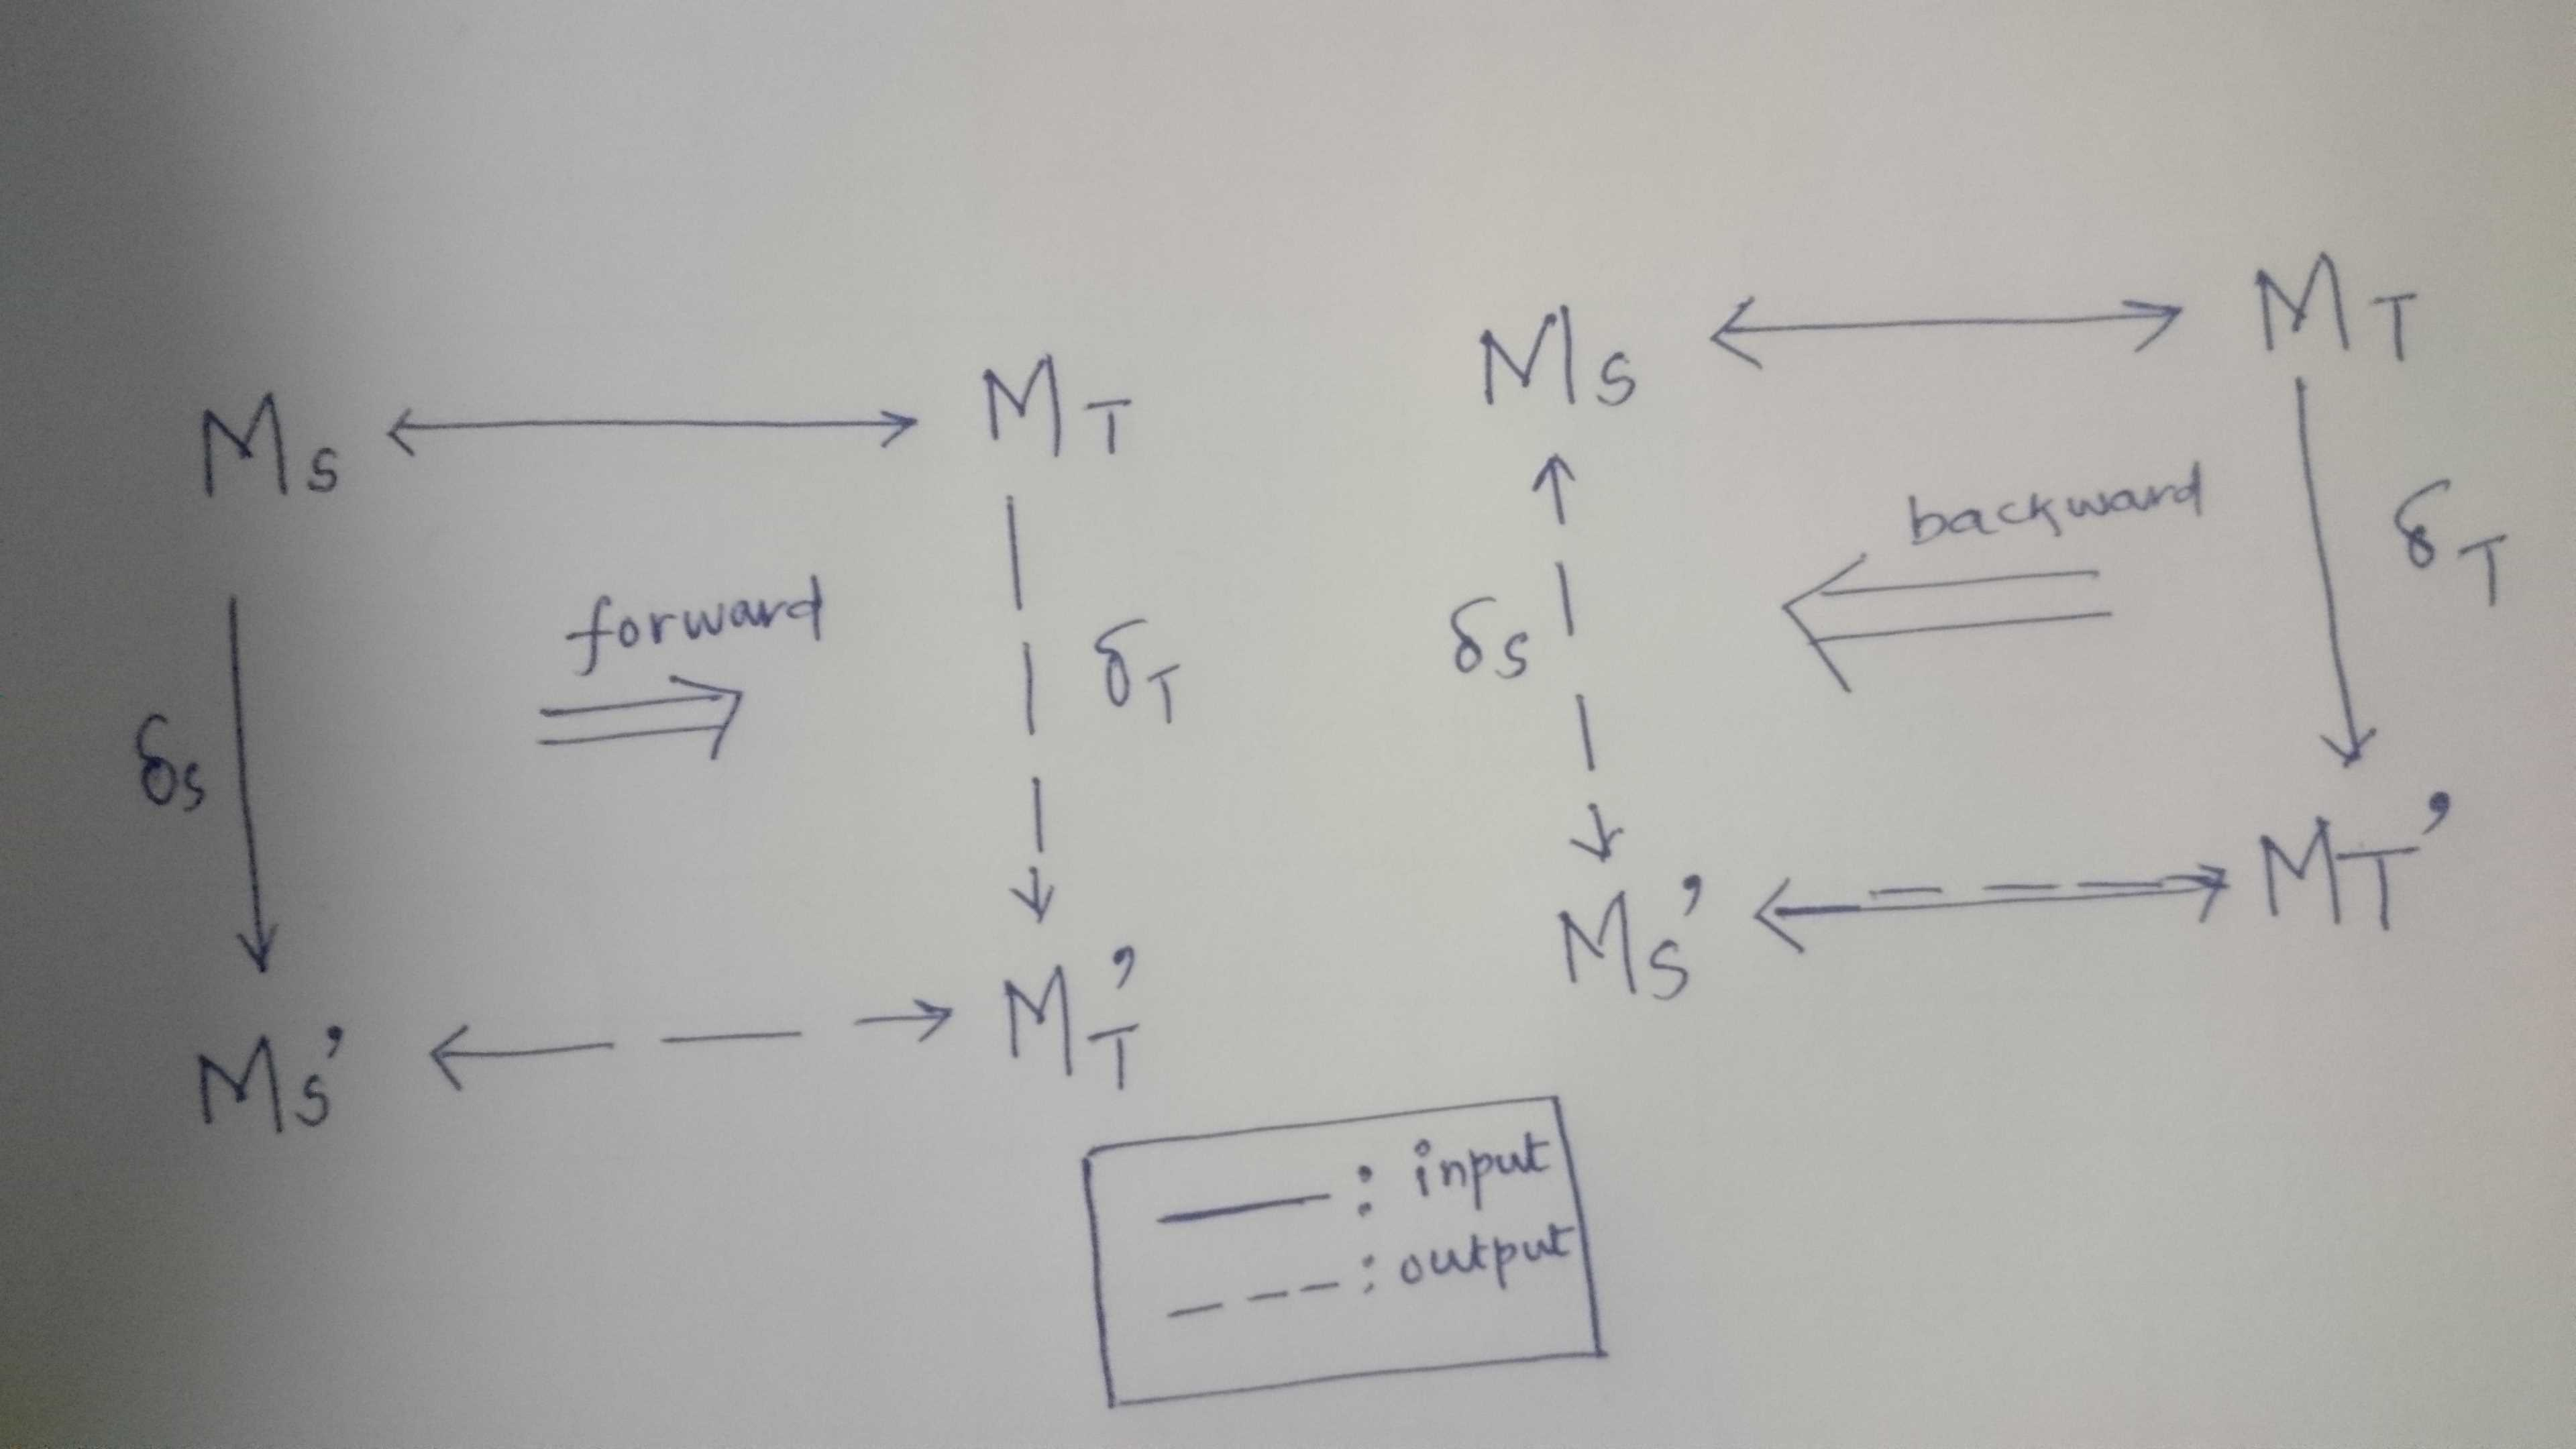
\includegraphics[width=1\textwidth]{figures/BX}
	\caption{Bidirectional Transformation}
	\label{fig:BX_Diagram}
\end{figure}

 



